\documentclass{article}

\usepackage{assign-style}

\usepackage{longtable}
\usepackage{tabu}

\setcoursetitle{CS345: Alorithms II}
\setassigncode{1}
\setauthname{Gurpreet Singh --- Nikita Awasthi}
\setauthroll{150259 --- 150453}

\begin{document}
\makeheader%

\section*{Time Plots}
\begin{margin}
    
    \begin{figure}[h!]
        \centering
        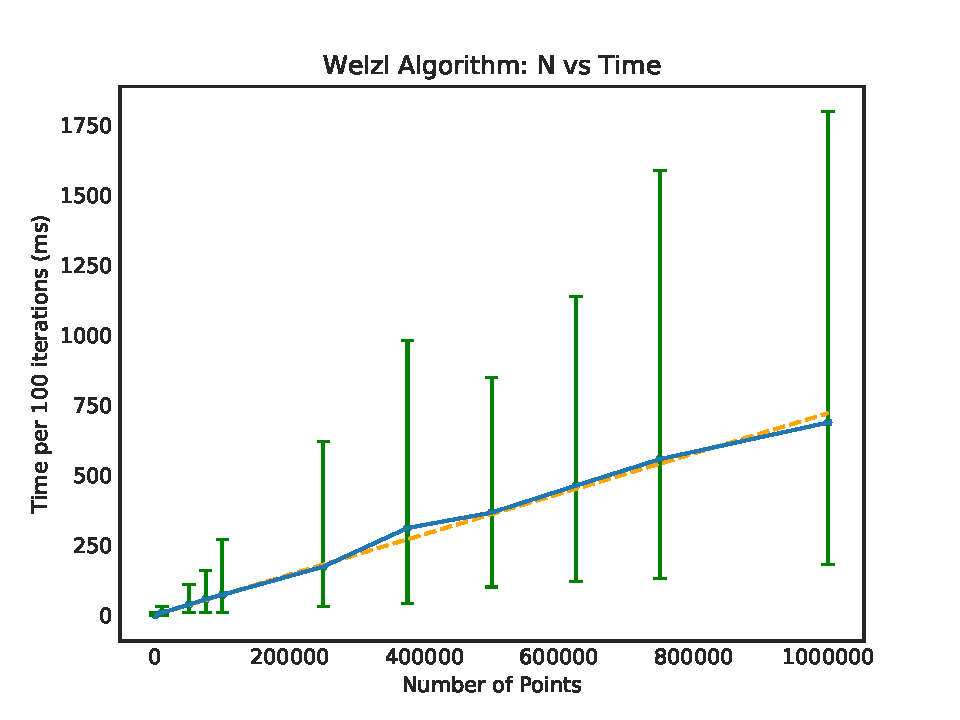
\includegraphics{plots/plot-welzl.pdf}
        \caption{Time vs Number of Points plot for the randomized algorithm}
        \label{fig:welzl}
    \end{figure}

    \begin{figure}[h!]
        \centering
        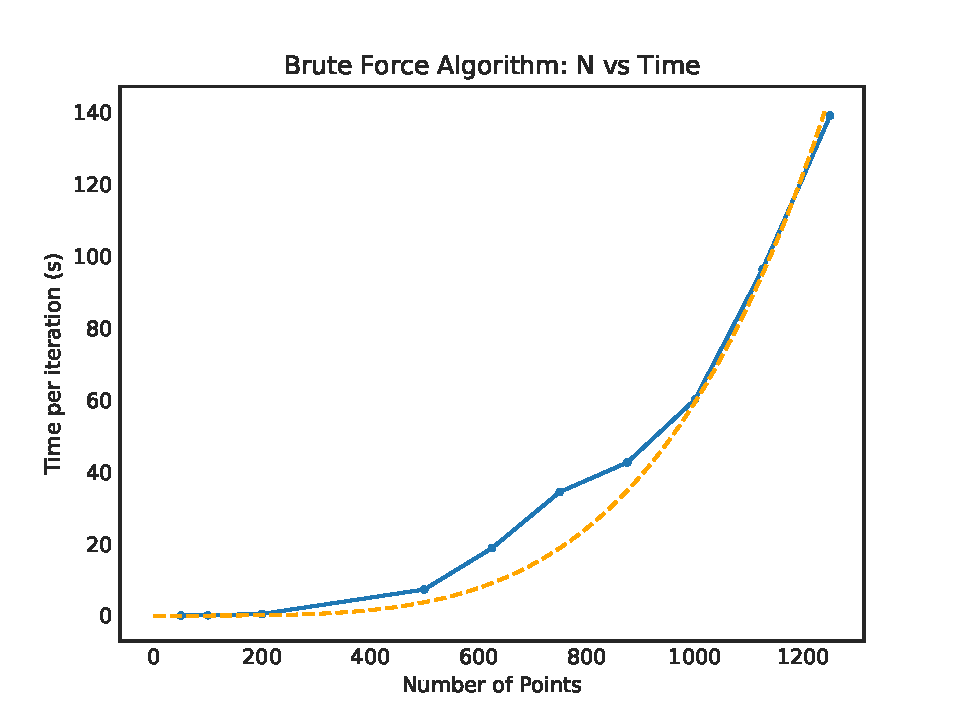
\includegraphics{plots/plot-brute.pdf}
        \caption{Time vs Number of Points plot for the brute force algorithm}
        \label{fig:brute}
    \end{figure}

\end{margin}

\section*{Informal Time Analysis}
\begin{margin}
    
    From the plot in figure~\ref{fig:welzl}, we can informally infer the time complexity of the randomized (Welzl) algorithm for finding the minimum enclosing circle. Looking at the plot points (mean of time taken) as well as the best-fit line, we can more or less say that the expected time is linear with the number of points \textit{i.e.} $\E{T(n)} = \bigO{n}$. \br%

    For the case of the brute force algorithm, we already know the time complexity \textit{i.e.} $\bigO{n^4}$, which is also visible from the plot in figure~\ref{fig:brute}.

\end{margin}

\section*{Distribution of Running Time}
\begin{margin}

    In order to find the best fit, we can minimize the difference between the expected time and the best fit line \textit{i.e.} For any best fit line, we aim to keep all the expected times as close to it as possible. Therefore, if we have the expected times for N points $\bset{p_n}_{n = 1}^{N}$, as $\bset{t_n}_{n = 1}^{N}$. Since it is only natural for us to take the best fit line passing through the origin, we consider this line to be $t = mp$. Therefore we have the optimization problem

    \begin{align*}
                    &\hat{m} = \argmax_{m} \sum_{n = 1}^{N} \bpara{t_n - mp_n}^{2} \\
        \implies    &\hat{m} = \frac{\sum_{n = 1}^{N} t_n p_n}{\sum_{n = 1}^{N} p_n^2}
    \end{align*} \br%

    Hence for our case, we obtain the best fit line as $t = 0.722415p$ (where $t$ is in $\mu s$). Using the same strategy, we can obtain a best fit for the brute force method. These best fit lines are show in the plots as orange dashed lines. \br%
   
    \clearpage

    For the case of Welzl's Algorithm, the number of times the running time deviates from the linear bound is given in the table below

    \def\arraystretch{1.5}
    \begin{longtabu}[h!]{c | c | c | c}
        \rowfont{\bfseries}
        Number of Points        &   Expected Time (in ms)   &   Standard Deviation (in ms)  &   \% of Iterations Violating $\bigO{n}$   \\
        \hline
        1000 	                &	0.6 	                &	2.37486841741 	            &	6 	                                    \\
        10000 	                &	7.5999998 	            &	6.34350053523 	            &	66 	                                    \\
        50000 	                &	37.0000039 	            &	19.8746152016 	            &	47 	                                    \\
        75000 	                &	55.90003 	            &	28.2876157729 	            &	45 	                                    \\
        100000 	                &	72.200042 	            &	42.6047372433 	            &	36 	                                    \\
        250000 	                &	172.899956 	            &	95.0608843646 	            &	32 	                                    \\
        375000 	                &	311.100128 	            &	170.680252527 	            &	55 	                                    \\
        500000 	                &	366.100015 	            &	188.906716206 	            &	42 	                                    \\
        625000 	                &	462.40037 	            &	226.262114926 	            &	42 	                                    \\
        750000 	                &	557.20017 	            &	324.192265785 	            &	43 	                                    \\
        1000000 	            &	688.30027 	            &	339.543487099 	            &	36 	                                    \\
    \end{longtabu}

    \begin{figure}[h!]
        \centering
        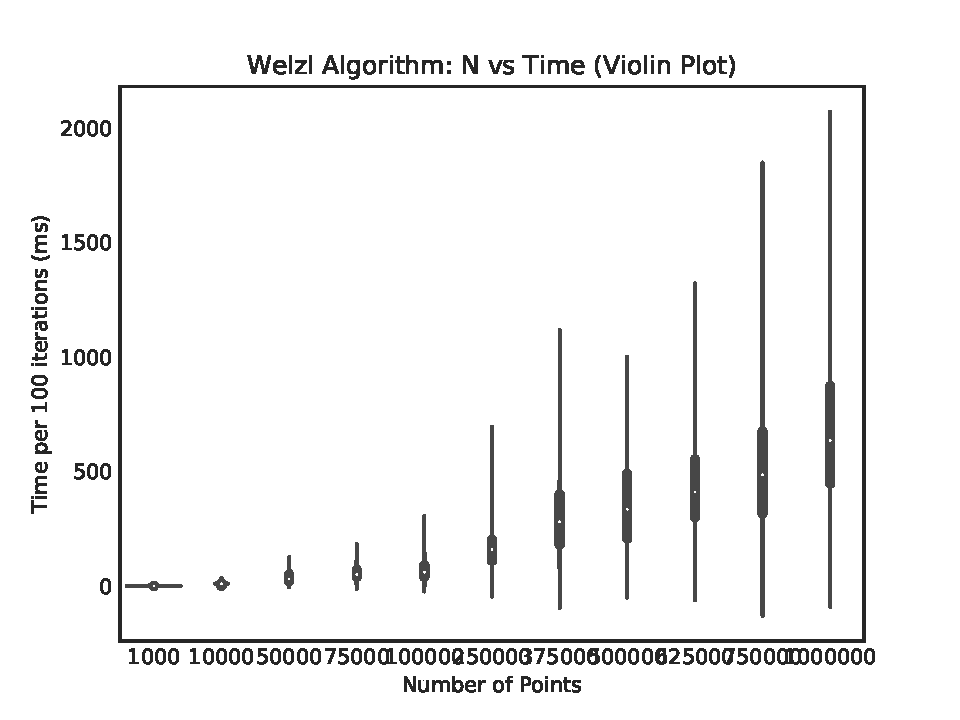
\includegraphics{plots/plot-welzl-violin.pdf}
        \caption{ViolinPlot of Time vs Number of Points for the Welzl Algorithm}
        \label{fig:welzl-violin}
    \end{figure}

    A few observations can be made about the percentage of points violating the linear bound

    \begin{itemize}
        \item \bt{The number of such points are very low for the first two cases.} This is because the LEDA library has very low precision in terms of time, ans thus we do not observe the precise time for less running time instances. This is most relevant for the first two cases, and hence mostly the time noted is very close to 0.
        \item \bt{The number of points is close 50\% for most number of points.} This might suggest that the linear bound is being broken by a lot of instances, however, it is not precisely so. Although the number of points may be high, however most of the points are very close to the expected running time, and hence the bound is not very severely affected. This can be visualized using the voilinplot given in figure~\ref{fig:welzl-violin}.
    \end{itemize}

\end{margin}

\end{document}
